\documentclass[twoside]{book}

% Packages required by doxygen
\usepackage{fixltx2e}
\usepackage{calc}
\usepackage{doxygen}
\usepackage[export]{adjustbox} % also loads graphicx
\usepackage{graphicx}
\usepackage[utf8]{inputenc}
\usepackage{makeidx}
\usepackage{multicol}
\usepackage{multirow}
\PassOptionsToPackage{warn}{textcomp}
\usepackage{textcomp}
\usepackage[nointegrals]{wasysym}
\usepackage[table]{xcolor}

% Font selection
\usepackage[T1]{fontenc}
\usepackage[scaled=.90]{helvet}
\usepackage{courier}
\usepackage{amssymb}
\usepackage{sectsty}
\renewcommand{\familydefault}{\sfdefault}
\allsectionsfont{%
  \fontseries{bc}\selectfont%
  \color{darkgray}%
}
\renewcommand{\DoxyLabelFont}{%
  \fontseries{bc}\selectfont%
  \color{darkgray}%
}
\newcommand{\+}{\discretionary{\mbox{\scriptsize$\hookleftarrow$}}{}{}}

% Page & text layout
\usepackage{geometry}
\geometry{%
  a4paper,%
  top=2.5cm,%
  bottom=2.5cm,%
  left=2.5cm,%
  right=2.5cm%
}
\tolerance=750
\hfuzz=15pt
\hbadness=750
\setlength{\emergencystretch}{15pt}
\setlength{\parindent}{0cm}
\setlength{\parskip}{3ex plus 2ex minus 2ex}
\makeatletter
\renewcommand{\paragraph}{%
  \@startsection{paragraph}{4}{0ex}{-1.0ex}{1.0ex}{%
    \normalfont\normalsize\bfseries\SS@parafont%
  }%
}
\renewcommand{\subparagraph}{%
  \@startsection{subparagraph}{5}{0ex}{-1.0ex}{1.0ex}{%
    \normalfont\normalsize\bfseries\SS@subparafont%
  }%
}
\makeatother

% Headers & footers
\usepackage{fancyhdr}
\pagestyle{fancyplain}
\fancyhead[LE]{\fancyplain{}{\bfseries\thepage}}
\fancyhead[CE]{\fancyplain{}{}}
\fancyhead[RE]{\fancyplain{}{\bfseries\leftmark}}
\fancyhead[LO]{\fancyplain{}{\bfseries\rightmark}}
\fancyhead[CO]{\fancyplain{}{}}
\fancyhead[RO]{\fancyplain{}{\bfseries\thepage}}
\fancyfoot[LE]{\fancyplain{}{}}
\fancyfoot[CE]{\fancyplain{}{}}
\fancyfoot[RE]{\fancyplain{}{\bfseries\scriptsize Generated by Doxygen }}
\fancyfoot[LO]{\fancyplain{}{\bfseries\scriptsize Generated by Doxygen }}
\fancyfoot[CO]{\fancyplain{}{}}
\fancyfoot[RO]{\fancyplain{}{}}
\renewcommand{\footrulewidth}{0.4pt}
\renewcommand{\chaptermark}[1]{%
  \markboth{#1}{}%
}
\renewcommand{\sectionmark}[1]{%
  \markright{\thesection\ #1}%
}

% Indices & bibliography
\usepackage{natbib}
\usepackage[titles]{tocloft}
\setcounter{tocdepth}{3}
\setcounter{secnumdepth}{5}
\makeindex

% Hyperlinks (required, but should be loaded last)
\usepackage{ifpdf}
\ifpdf
  \usepackage[pdftex,pagebackref=true]{hyperref}
\else
  \usepackage[ps2pdf,pagebackref=true]{hyperref}
\fi
\hypersetup{%
  colorlinks=true,%
  linkcolor=blue,%
  citecolor=blue,%
  unicode%
}

% Custom commands
\newcommand{\clearemptydoublepage}{%
  \newpage{\pagestyle{empty}\cleardoublepage}%
}

\usepackage{caption}
\captionsetup{labelsep=space,justification=centering,font={bf},singlelinecheck=off,skip=4pt,position=top}

%===== C O N T E N T S =====

\begin{document}

% Titlepage & ToC
\hypersetup{pageanchor=false,
             bookmarksnumbered=true,
             pdfencoding=unicode
            }
\pagenumbering{alph}
\begin{titlepage}
\vspace*{7cm}
\begin{center}%
{\Large Symbolic Regression Team 5 \\[1ex]\large 1.\+0 }\\
\vspace*{1cm}
{\large Generated by Doxygen 1.8.13}\\
\end{center}
\end{titlepage}
\clearemptydoublepage
\pagenumbering{roman}
\tableofcontents
\clearemptydoublepage
\pagenumbering{arabic}
\hypersetup{pageanchor=true}

%--- Begin generated contents ---
\chapter{Symbolic-\/\+Regression}
\label{md_README}
\Hypertarget{md_README}
Goal \+: Find the best approximation Content \+: 2 class --$>$ \hyperlink{classNode}{Node} \+: Treat the tree of the formula --$>$ \hyperlink{classEvolution}{Evolution} \+: Modify the function


\begin{DoxyItemize}
\item \hyperlink{classNode}{Node} \+: 3 attributs (2 \hyperlink{classNode}{Node} and 1 char$\ast$)
\begin{DoxyItemize}
\item Constructor \+: \hyperlink{classNode}{Node(\+Node$\ast$ lc, Node$\ast$ rc, std\+::string v)} et copy constructor; plus destructor et getters
\item int node\+\_\+result() \+: for have the result of the formula
\item int node\+\_\+result(int x1, int x2) \+: for have the result of the formula with different value at the end of the tree
\item std\+::string node\+\_\+formula() \+: give the formula of the tree
\end{DoxyItemize}
\item \hyperlink{classEvolution}{Evolution} \+: n attributs () -\/ Use class \hyperlink{classNode}{Node}
\begin{DoxyItemize}
\item Node$\ast$ replication(\+Node root, int number\+\_\+of\+\_\+child) \+: for create number\+\_\+of\+\_\+child children to the parent\textquotesingle{}s formula
\item void mutation(\+Node position, Node root) \+: choose a mutation to a given node of the formula
\item \hyperlink{classNode}{Node} insertion(\+Node parent, Node root) \+: make the mutation \textquotesingle{}insertion\textquotesingle{} at a given place of the formula
\item \hyperlink{classNode}{Node} deletion(\+Node parent, Node root) \+: make the mutation \textquotesingle{}deletion\textquotesingle{} at a given place of the formula
\item \hyperlink{classNode}{Node} replacement(\+Node parent, Node root) \+: make the mutation \textquotesingle{}deletion\textquotesingle{} at a given node of the formula
\item int fitness(\+Node tree, int$\ast$ donnee) \+: calculation of the fitness of a formula
\item \hyperlink{classNode}{Node} $\ast$ comparative\+\_\+fitness (\hyperlink{classNode}{Node} root, Node$\ast$ childre\+\_\+tab, int number\+\_\+of\+\_\+child, int$\ast$ donnee) \+: choose the best children of the formula 
\end{DoxyItemize}
\end{DoxyItemize}
\chapter{Class Index}
\section{Class List}
Here are the classes, structs, unions and interfaces with brief descriptions\+:\begin{DoxyCompactList}
\item\contentsline{section}{\hyperlink{classEvolution}{Evolution} }{\pageref{classEvolution}}{}
\item\contentsline{section}{\hyperlink{classNode}{Node} }{\pageref{classNode}}{}
\end{DoxyCompactList}

\chapter{Class Documentation}
\hypertarget{classEvolution}{}\section{Evolution Class Reference}
\label{classEvolution}\index{Evolution@{Evolution}}


Collaboration diagram for Evolution\+:
\nopagebreak
\begin{figure}[H]
\begin{center}
\leavevmode
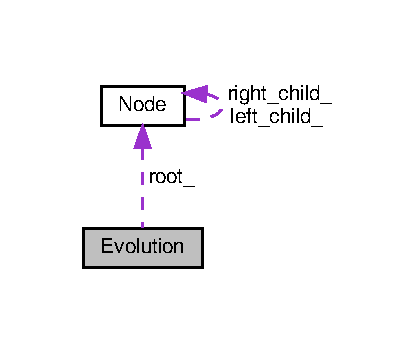
\includegraphics[width=200pt]{classEvolution__coll__graph}
\end{center}
\end{figure}
\subsection*{Public Member Functions}
\begin{DoxyCompactItemize}
\item 
\mbox{\Hypertarget{classEvolution_a0502489a07abf6f9bbc72cfcf4767c3e}\label{classEvolution_a0502489a07abf6f9bbc72cfcf4767c3e}} 
\hyperlink{classEvolution_a0502489a07abf6f9bbc72cfcf4767c3e}{Evolution} (\hyperlink{classNode}{Node} $\ast$node, std\+::string \hyperlink{classEvolution_afb925477cdd6c8703304a037208e64e1}{data})
\begin{DoxyCompactList}\small\item\em Instantiates an \hyperlink{classEvolution}{Evolution} object with a base \hyperlink{classNode}{Node} node and a path to a csv file. \end{DoxyCompactList}\item 
\mbox{\Hypertarget{classEvolution_acb98a24071fe199644585c6192bed933}\label{classEvolution_acb98a24071fe199644585c6192bed933}} 
std\+::vector$<$ float $>$ \hyperlink{classEvolution_acb98a24071fe199644585c6192bed933}{evolution} (int number\+\_\+of\+\_\+cycles, int number\+\_\+of\+\_\+children)
\begin{DoxyCompactList}\small\item\em Starts the whole algorithm of symbolic regression with number\+\_\+of\+\_\+cycles cycles and number\+\_\+of\+\_\+children children for each cycle. \end{DoxyCompactList}\item 
\mbox{\Hypertarget{classEvolution_a83182c1db463268e933cc0ca9c46d056}\label{classEvolution_a83182c1db463268e933cc0ca9c46d056}} 
\hyperlink{classNode}{Node} $\ast$ \hyperlink{classEvolution_a83182c1db463268e933cc0ca9c46d056}{root} ()
\begin{DoxyCompactList}\small\item\em Returns the current base \hyperlink{classNode}{Node} of the future mutants. \end{DoxyCompactList}\item 
\mbox{\Hypertarget{classEvolution_a98ea253854899bea05cdb0c13a7eb85a}\label{classEvolution_a98ea253854899bea05cdb0c13a7eb85a}} 
std\+::vector$<$ \hyperlink{classNode}{Node} $\ast$ $>$ \hyperlink{classEvolution_a98ea253854899bea05cdb0c13a7eb85a}{mutant\+\_\+children} ()
\begin{DoxyCompactList}\small\item\em Returns the vector of mutants. \end{DoxyCompactList}\item 
\mbox{\Hypertarget{classEvolution_afb925477cdd6c8703304a037208e64e1}\label{classEvolution_afb925477cdd6c8703304a037208e64e1}} 
std\+::vector$<$ std\+::vector$<$ int $>$ $>$ \hyperlink{classEvolution_afb925477cdd6c8703304a037208e64e1}{data} ()
\begin{DoxyCompactList}\small\item\em Returns the vector containing the data of the csv file. \end{DoxyCompactList}\item 
\mbox{\Hypertarget{classEvolution_a81a8234ea0ed97fe84f4cf6a80f37f44}\label{classEvolution_a81a8234ea0ed97fe84f4cf6a80f37f44}} 
std\+::vector$<$ float $>$ \hyperlink{classEvolution_a81a8234ea0ed97fe84f4cf6a80f37f44}{fitnesses} ()
\begin{DoxyCompactList}\small\item\em Returns the vector of computed fitnesses per mutants. \end{DoxyCompactList}\item 
\mbox{\Hypertarget{classEvolution_acd01c2f27d399ccece49258e0a29ba0b}\label{classEvolution_acd01c2f27d399ccece49258e0a29ba0b}} 
void \hyperlink{classEvolution_acd01c2f27d399ccece49258e0a29ba0b}{set\+\_\+node} (\hyperlink{classNode}{Node} $\ast$node)
\begin{DoxyCompactList}\small\item\em Changes the base \hyperlink{classNode}{Node} of the future mutants. \end{DoxyCompactList}\item 
\mbox{\Hypertarget{classEvolution_ac5e3ce959ccf663c17e2930ea508e6a5}\label{classEvolution_ac5e3ce959ccf663c17e2930ea508e6a5}} 
void \hyperlink{classEvolution_ac5e3ce959ccf663c17e2930ea508e6a5}{set\+\_\+data} (std\+::string \hyperlink{classEvolution_afb925477cdd6c8703304a037208e64e1}{data})
\begin{DoxyCompactList}\small\item\em Changes the csv file. \end{DoxyCompactList}\end{DoxyCompactItemize}
\subsection*{Protected Member Functions}
\begin{DoxyCompactItemize}
\item 
\mbox{\Hypertarget{classEvolution_aac3850387f35657c75c6deaf1e711538}\label{classEvolution_aac3850387f35657c75c6deaf1e711538}} 
std\+::vector$<$ \hyperlink{classNode}{Node} $\ast$ $>$ \hyperlink{classEvolution_aac3850387f35657c75c6deaf1e711538}{replication\+\_\+} (int number\+\_\+of\+\_\+children)
\begin{DoxyCompactList}\small\item\em Makes a vector of number\+\_\+of\+\_\+children clones from the base \hyperlink{classNode}{Node}. \end{DoxyCompactList}\item 
\mbox{\Hypertarget{classEvolution_ae4ec9688c4d948d9c31f29069804b0b0}\label{classEvolution_ae4ec9688c4d948d9c31f29069804b0b0}} 
void \hyperlink{classEvolution_ae4ec9688c4d948d9c31f29069804b0b0}{mutation\+\_\+} (\hyperlink{classNode}{Node} $\ast$position, \hyperlink{classNode}{Node} $\ast$\hyperlink{classEvolution_a83182c1db463268e933cc0ca9c46d056}{root}, int id)
\begin{DoxyCompactList}\small\item\em Makes a mutation on a precise \hyperlink{classNode}{Node} of a future mutant. \end{DoxyCompactList}\item 
\mbox{\Hypertarget{classEvolution_a436adadb0c98f7c12ae7be370b030a27}\label{classEvolution_a436adadb0c98f7c12ae7be370b030a27}} 
void \hyperlink{classEvolution_a436adadb0c98f7c12ae7be370b030a27}{insertion\+\_\+} (\hyperlink{classNode}{Node} $\ast$position, \hyperlink{classNode}{Node} $\ast$parent, int id)
\begin{DoxyCompactList}\small\item\em Makes a mutation of type insertion on a precise \hyperlink{classNode}{Node} of a future mutant. \end{DoxyCompactList}\item 
\mbox{\Hypertarget{classEvolution_a7832fd571fde0712015e5e50f5134abc}\label{classEvolution_a7832fd571fde0712015e5e50f5134abc}} 
void \hyperlink{classEvolution_a7832fd571fde0712015e5e50f5134abc}{deletion\+\_\+} (\hyperlink{classNode}{Node} $\ast$position, \hyperlink{classNode}{Node} $\ast$parent, int id)
\begin{DoxyCompactList}\small\item\em Makes a mutation of type deletion on a precise \hyperlink{classNode}{Node} of a future mutant. \end{DoxyCompactList}\item 
\mbox{\Hypertarget{classEvolution_aca700a0c053e1d6665aa184c773f3b9a}\label{classEvolution_aca700a0c053e1d6665aa184c773f3b9a}} 
void \hyperlink{classEvolution_aca700a0c053e1d6665aa184c773f3b9a}{replacement\+\_\+} (\hyperlink{classNode}{Node} $\ast$position, \hyperlink{classNode}{Node} $\ast$parent, int id)
\begin{DoxyCompactList}\small\item\em Makes a mutation of type replacement on a precise \hyperlink{classNode}{Node} of a future mutant. \end{DoxyCompactList}\item 
\mbox{\Hypertarget{classEvolution_ae58e042dadbc735ede6f295050348348}\label{classEvolution_ae58e042dadbc735ede6f295050348348}} 
void \hyperlink{classEvolution_ae58e042dadbc735ede6f295050348348}{replacement\+\_\+leaf\+\_\+management\+\_\+} (\hyperlink{classNode}{Node} $\ast$position, \hyperlink{classNode}{Node} $\ast$parent, \hyperlink{classNode}{Node} $\ast$new\+\_\+node\+\_\+1, \hyperlink{classNode}{Node} $\ast$new\+\_\+node\+\_\+2, int index\+\_\+1, int index\+\_\+2, int n, int id)
\begin{DoxyCompactList}\small\item\em Auxiliary function to manage a replacement on a leaf \hyperlink{classNode}{Node}. \end{DoxyCompactList}\item 
\mbox{\Hypertarget{classEvolution_ab0df05e5d9386e6c4e28fedf4e714ba2}\label{classEvolution_ab0df05e5d9386e6c4e28fedf4e714ba2}} 
void \hyperlink{classEvolution_ab0df05e5d9386e6c4e28fedf4e714ba2}{replacement\+\_\+and\+\_\+management\+\_\+} (\hyperlink{classNode}{Node} $\ast$position, \hyperlink{classNode}{Node} $\ast$parent, \hyperlink{classNode}{Node} $\ast$new\+\_\+node\+\_\+1, \hyperlink{classNode}{Node} $\ast$new\+\_\+node\+\_\+2, int index\+\_\+1, int index\+\_\+2, int n, int id)
\begin{DoxyCompactList}\small\item\em Auxiliary function to manage a replacement on an A\+ND \hyperlink{classNode}{Node}. \end{DoxyCompactList}\item 
\mbox{\Hypertarget{classEvolution_aa5bfb77427e28dfb74a5743459492204}\label{classEvolution_aa5bfb77427e28dfb74a5743459492204}} 
void \hyperlink{classEvolution_aa5bfb77427e28dfb74a5743459492204}{replacement\+\_\+or\+\_\+management\+\_\+} (\hyperlink{classNode}{Node} $\ast$position, \hyperlink{classNode}{Node} $\ast$parent, \hyperlink{classNode}{Node} $\ast$new\+\_\+node\+\_\+1, \hyperlink{classNode}{Node} $\ast$new\+\_\+node\+\_\+2, int index\+\_\+1, int index\+\_\+2, int n, int id)
\begin{DoxyCompactList}\small\item\em Auxiliary function to manage a replacement on an OR \hyperlink{classNode}{Node}. \end{DoxyCompactList}\item 
\mbox{\Hypertarget{classEvolution_a4686436a67c724b9e682b92cc48e24c5}\label{classEvolution_a4686436a67c724b9e682b92cc48e24c5}} 
void \hyperlink{classEvolution_a4686436a67c724b9e682b92cc48e24c5}{replacement\+\_\+not\+\_\+management\+\_\+} (\hyperlink{classNode}{Node} $\ast$position, \hyperlink{classNode}{Node} $\ast$parent, \hyperlink{classNode}{Node} $\ast$new\+\_\+node\+\_\+1, \hyperlink{classNode}{Node} $\ast$new\+\_\+node\+\_\+2, int index\+\_\+1, int index\+\_\+2, int n, int id)
\begin{DoxyCompactList}\small\item\em Auxiliary function to manage a replacement on a N\+OT \hyperlink{classNode}{Node}. \end{DoxyCompactList}\item 
\mbox{\Hypertarget{classEvolution_a9863357caa544557ef14fc1c63476dd5}\label{classEvolution_a9863357caa544557ef14fc1c63476dd5}} 
float \hyperlink{classEvolution_a9863357caa544557ef14fc1c63476dd5}{compute\+\_\+fitness\+\_\+} (\hyperlink{classNode}{Node} $\ast$node)
\begin{DoxyCompactList}\small\item\em Computes and returns the fitness for one \hyperlink{classNode}{Node}. \end{DoxyCompactList}\item 
\mbox{\Hypertarget{classEvolution_aa727c218cb791aac6204434a1c648e84}\label{classEvolution_aa727c218cb791aac6204434a1c648e84}} 
void \hyperlink{classEvolution_aa727c218cb791aac6204434a1c648e84}{compare\+\_\+fitness\+\_\+} ()
\begin{DoxyCompactList}\small\item\em Compares all mutants\textquotesingle{} fitnesses and if one of them has a better fitness than the base \hyperlink{classNode}{Node}, it becomes the new base \hyperlink{classNode}{Node} for the following cycle. \end{DoxyCompactList}\item 
\mbox{\Hypertarget{classEvolution_a593cd110aa18282f2d03b8539fc8db7f}\label{classEvolution_a593cd110aa18282f2d03b8539fc8db7f}} 
void \hyperlink{classEvolution_a593cd110aa18282f2d03b8539fc8db7f}{apoptosis\+\_\+} (\hyperlink{classNode}{Node} $\ast$node, int id)
\begin{DoxyCompactList}\small\item\em Deletes a \hyperlink{classNode}{Node} with its children. \end{DoxyCompactList}\item 
\mbox{\Hypertarget{classEvolution_ac22e226d32fe53774b437c51903816db}\label{classEvolution_ac22e226d32fe53774b437c51903816db}} 
\hyperlink{classNode}{Node} $\ast$ \hyperlink{classEvolution_ac22e226d32fe53774b437c51903816db}{get\+\_\+parent\+\_\+node\+\_\+} (\hyperlink{classNode}{Node} $\ast$position, \hyperlink{classNode}{Node} $\ast$\hyperlink{classEvolution_a83182c1db463268e933cc0ca9c46d056}{root})
\begin{DoxyCompactList}\small\item\em Returns a pointer pointing on the parent of the \hyperlink{classNode}{Node} position. \end{DoxyCompactList}\item 
\mbox{\Hypertarget{classEvolution_a9d5f4998a7ec21ea2a2bec87b89d26ec}\label{classEvolution_a9d5f4998a7ec21ea2a2bec87b89d26ec}} 
int \hyperlink{classEvolution_a9d5f4998a7ec21ea2a2bec87b89d26ec}{left\+\_\+or\+\_\+right\+\_\+child\+\_\+} (\hyperlink{classNode}{Node} $\ast$position, \hyperlink{classNode}{Node} $\ast$parent)
\begin{DoxyCompactList}\small\item\em Returns -\/1 if the \hyperlink{classNode}{Node} position isn\textquotesingle{}t a child, 0 if the \hyperlink{classNode}{Node} position is a left child and 1 if the \hyperlink{classNode}{Node} position is a right child. \end{DoxyCompactList}\item 
\mbox{\Hypertarget{classEvolution_a94143bdc521fa73e8f0fa94a017c5217}\label{classEvolution_a94143bdc521fa73e8f0fa94a017c5217}} 
\hyperlink{classNode}{Node} $\ast$ \hyperlink{classEvolution_a94143bdc521fa73e8f0fa94a017c5217}{node\+\_\+at\+\_\+path\+\_\+} (\hyperlink{classNode}{Node} $\ast$node, std\+::string path)
\begin{DoxyCompactList}\small\item\em Returns the \hyperlink{classNode}{Node} on which the mutation will occur. \end{DoxyCompactList}\item 
\mbox{\Hypertarget{classEvolution_a983dff352ca0f1587db8b259a2e3ae67}\label{classEvolution_a983dff352ca0f1587db8b259a2e3ae67}} 
std\+::string \hyperlink{classEvolution_a983dff352ca0f1587db8b259a2e3ae67}{generate\+\_\+path\+\_\+} ()
\begin{DoxyCompactList}\small\item\em Generates and returns a randomly generated path to the \hyperlink{classNode}{Node} on which the mutation will occur. \end{DoxyCompactList}\item 
\mbox{\Hypertarget{classEvolution_a89200535246f4a1de3495a6e47d6fc1a}\label{classEvolution_a89200535246f4a1de3495a6e47d6fc1a}} 
std\+::vector$<$ std\+::vector$<$ int $>$ $>$ \hyperlink{classEvolution_a89200535246f4a1de3495a6e47d6fc1a}{parse\+\_\+data\+\_\+} (std\+::string data\+\_\+to\+\_\+parse)
\begin{DoxyCompactList}\small\item\em Generates and returns a vector containing the data of the csv file. \end{DoxyCompactList}\item 
\mbox{\Hypertarget{classEvolution_abd53fdd9448e1477789d7a338f526677}\label{classEvolution_abd53fdd9448e1477789d7a338f526677}} 
void \hyperlink{classEvolution_abd53fdd9448e1477789d7a338f526677}{generate\+\_\+used\+\_\+operands\+\_\+} (\hyperlink{classNode}{Node} $\ast$\hyperlink{classEvolution_a83182c1db463268e933cc0ca9c46d056}{root}, std\+::vector$<$ std\+::string $>$ \&sub\+\_\+used\+\_\+operands)
\begin{DoxyCompactList}\small\item\em Generates a vector of vector of unusable genes for each future mutant (only one copy of the gene for one formula) \end{DoxyCompactList}\item 
\mbox{\Hypertarget{classEvolution_a176d3769f71445ea1ad01c1f15c32228}\label{classEvolution_a176d3769f71445ea1ad01c1f15c32228}} 
void \hyperlink{classEvolution_a176d3769f71445ea1ad01c1f15c32228}{generate\+\_\+operands\+\_\+} (int number)
\begin{DoxyCompactList}\small\item\em Generates a vector of vector of usable genes for each future mutant. \end{DoxyCompactList}\item 
\mbox{\Hypertarget{classEvolution_afcab6985218702a13538e847e0299650}\label{classEvolution_afcab6985218702a13538e847e0299650}} 
void \hyperlink{classEvolution_afcab6985218702a13538e847e0299650}{operands\+\_\+to\+\_\+used\+\_\+} (int index, int id)
\begin{DoxyCompactList}\small\item\em When a gene is used, it is transfered to the corresponding vector of no more usable genes. \end{DoxyCompactList}\item 
\mbox{\Hypertarget{classEvolution_a65a44933413f08e42476bd4effec5943}\label{classEvolution_a65a44933413f08e42476bd4effec5943}} 
void \hyperlink{classEvolution_a65a44933413f08e42476bd4effec5943}{used\+\_\+to\+\_\+operands\+\_\+} (int index, int id)
\begin{DoxyCompactList}\small\item\em When a \hyperlink{classNode}{Node} is deleted, its genes are transfered to the corresponding vector of usable genes. \end{DoxyCompactList}\item 
\mbox{\Hypertarget{classEvolution_a6fbea5d647dc45271386d75636deecba}\label{classEvolution_a6fbea5d647dc45271386d75636deecba}} 
void \hyperlink{classEvolution_a6fbea5d647dc45271386d75636deecba}{re\+\_\+operands\+\_\+to\+\_\+used\+\_\+} (\hyperlink{classNode}{Node} $\ast$node, int id)
\begin{DoxyCompactList}\small\item\em Same as operands\+\_\+to\+\_\+used\+\_\+ but with a \hyperlink{classNode}{Node} as parameter. \end{DoxyCompactList}\end{DoxyCompactItemize}
\subsection*{Protected Attributes}
\begin{DoxyCompactItemize}
\item 
\mbox{\Hypertarget{classEvolution_a80b78a81e6a45625ac7ec9385cdb5476}\label{classEvolution_a80b78a81e6a45625ac7ec9385cdb5476}} 
std\+::vector$<$ \hyperlink{classNode}{Node} $\ast$ $>$ {\bfseries mutant\+\_\+children\+\_\+}
\item 
\mbox{\Hypertarget{classEvolution_a2d2222876a0c4ccbd084a2397aa8dd77}\label{classEvolution_a2d2222876a0c4ccbd084a2397aa8dd77}} 
\hyperlink{classNode}{Node} $\ast$ \hyperlink{classEvolution_a2d2222876a0c4ccbd084a2397aa8dd77}{root\+\_\+}
\begin{DoxyCompactList}\small\item\em Vector of mutated clones. \end{DoxyCompactList}\item 
\mbox{\Hypertarget{classEvolution_afce3ea47630dccad2760e3acae36e73e}\label{classEvolution_afce3ea47630dccad2760e3acae36e73e}} 
std\+::string \hyperlink{classEvolution_afce3ea47630dccad2760e3acae36e73e}{path\+\_\+}
\begin{DoxyCompactList}\small\item\em Base \hyperlink{classNode}{Node} from which will be generated the clones to be mutated. \end{DoxyCompactList}\item 
\mbox{\Hypertarget{classEvolution_aa7234f8d9153dbbf9103d17729064ae0}\label{classEvolution_aa7234f8d9153dbbf9103d17729064ae0}} 
std\+::vector$<$ std\+::vector$<$ int $>$ $>$ \hyperlink{classEvolution_aa7234f8d9153dbbf9103d17729064ae0}{data\+\_\+}
\begin{DoxyCompactList}\small\item\em The path to the actual \hyperlink{classNode}{Node} to mutate. \end{DoxyCompactList}\item 
\mbox{\Hypertarget{classEvolution_a9b9e7d53412a518ce862a0abfc06d149}\label{classEvolution_a9b9e7d53412a518ce862a0abfc06d149}} 
std\+::vector$<$ float $>$ \hyperlink{classEvolution_a9b9e7d53412a518ce862a0abfc06d149}{fitnesses\+\_\+}
\begin{DoxyCompactList}\small\item\em Vector containing the data of the csv file. \end{DoxyCompactList}\end{DoxyCompactItemize}


\subsection{Detailed Description}


Definition at line 3 of file Evolution.\+h.



The documentation for this class was generated from the following files\+:\begin{DoxyCompactItemize}
\item 
Evolution.\+h\item 
Evolution.\+cpp\end{DoxyCompactItemize}

\hypertarget{classNode}{}\section{Node Class Reference}
\label{classNode}\index{Node@{Node}}


Collaboration diagram for Node\+:
\nopagebreak
\begin{figure}[H]
\begin{center}
\leavevmode
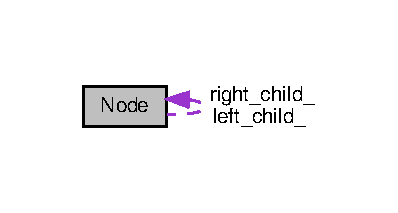
\includegraphics[width=191pt]{classNode__coll__graph}
\end{center}
\end{figure}
\subsection*{Public Member Functions}
\begin{DoxyCompactItemize}
\item 
\mbox{\Hypertarget{classNode_aeeda019b6480a7ae5713890f802b7055}\label{classNode_aeeda019b6480a7ae5713890f802b7055}} 
{\bfseries Node} (\hyperlink{classNode}{Node} $\ast$lc, \hyperlink{classNode}{Node} $\ast$rc, std\+::string v)
\item 
\mbox{\Hypertarget{classNode_a0089889f0d4e22f1cbb707ca9e1c27ea}\label{classNode_a0089889f0d4e22f1cbb707ca9e1c27ea}} 
\hyperlink{classNode_a0089889f0d4e22f1cbb707ca9e1c27ea}{Node} (\hyperlink{classNode}{Node} \&root)
\begin{DoxyCompactList}\small\item\em Makes a deep copy of the \hyperlink{classNode}{Node} including its children. \end{DoxyCompactList}\item 
\mbox{\Hypertarget{classNode_a1326a789dd57a0219d6c4927573c4965}\label{classNode_a1326a789dd57a0219d6c4927573c4965}} 
\hyperlink{classNode}{Node} $\ast$ \hyperlink{classNode_a1326a789dd57a0219d6c4927573c4965}{left\+\_\+child} ()
\begin{DoxyCompactList}\small\item\em Returns the pointer on the left child. \end{DoxyCompactList}\item 
\mbox{\Hypertarget{classNode_a3c9dba1de9c55937d71598d4ba06314b}\label{classNode_a3c9dba1de9c55937d71598d4ba06314b}} 
\hyperlink{classNode}{Node} $\ast$ \hyperlink{classNode_a3c9dba1de9c55937d71598d4ba06314b}{right\+\_\+child} ()
\begin{DoxyCompactList}\small\item\em Returns the pointer on the right child. \end{DoxyCompactList}\item 
\mbox{\Hypertarget{classNode_a932c934ef9fe76a2839db304529c7769}\label{classNode_a932c934ef9fe76a2839db304529c7769}} 
std\+::string \hyperlink{classNode_a932c934ef9fe76a2839db304529c7769}{value} ()
\begin{DoxyCompactList}\small\item\em Returns the value of the \hyperlink{classNode}{Node}. \end{DoxyCompactList}\item 
\mbox{\Hypertarget{classNode_a50c34dde7898f3992c72eef3df00917b}\label{classNode_a50c34dde7898f3992c72eef3df00917b}} 
void \hyperlink{classNode_a50c34dde7898f3992c72eef3df00917b}{set\+\_\+left\+\_\+child} (\hyperlink{classNode}{Node} $\ast$lc)
\begin{DoxyCompactList}\small\item\em Changes the pointer pointing on the left child. \end{DoxyCompactList}\item 
\mbox{\Hypertarget{classNode_a85f67c5236d38be3e552551b408c2399}\label{classNode_a85f67c5236d38be3e552551b408c2399}} 
void \hyperlink{classNode_a85f67c5236d38be3e552551b408c2399}{set\+\_\+right\+\_\+child} (\hyperlink{classNode}{Node} $\ast$rc)
\begin{DoxyCompactList}\small\item\em Changes the pointer pointing on the right child. \end{DoxyCompactList}\item 
\mbox{\Hypertarget{classNode_af93bfefb945b9cf6acf3ad1361c4810f}\label{classNode_af93bfefb945b9cf6acf3ad1361c4810f}} 
void \hyperlink{classNode_af93bfefb945b9cf6acf3ad1361c4810f}{set\+\_\+value} (std\+::string s)
\begin{DoxyCompactList}\small\item\em Changes the value of the current \hyperlink{classNode}{Node}. \end{DoxyCompactList}\item 
\mbox{\Hypertarget{classNode_adf58a08bb7b8f8247b5a7db7339e6385}\label{classNode_adf58a08bb7b8f8247b5a7db7339e6385}} 
int \hyperlink{classNode_adf58a08bb7b8f8247b5a7db7339e6385}{node\+\_\+result} (std\+::vector$<$ int $>$ x)
\begin{DoxyCompactList}\small\item\em Computes and returns the results of one line of the csv file at the current \hyperlink{classNode}{Node}. \end{DoxyCompactList}\item 
\mbox{\Hypertarget{classNode_ac7dee6a30adfb99120189f280e61bc4b}\label{classNode_ac7dee6a30adfb99120189f280e61bc4b}} 
std\+::string \hyperlink{classNode_ac7dee6a30adfb99120189f280e61bc4b}{node\+\_\+formula} ()
\begin{DoxyCompactList}\small\item\em Computes and returns the formula at the current \hyperlink{classNode}{Node}. \end{DoxyCompactList}\end{DoxyCompactItemize}
\subsection*{Protected Attributes}
\begin{DoxyCompactItemize}
\item 
\mbox{\Hypertarget{classNode_a5ee0db484771d8654c32e7863fba292e}\label{classNode_a5ee0db484771d8654c32e7863fba292e}} 
\hyperlink{classNode}{Node} $\ast$ {\bfseries left\+\_\+child\+\_\+}
\item 
\mbox{\Hypertarget{classNode_abf180145dff7ffce95b3b39bfe24d2f6}\label{classNode_abf180145dff7ffce95b3b39bfe24d2f6}} 
\hyperlink{classNode}{Node} $\ast$ \hyperlink{classNode_abf180145dff7ffce95b3b39bfe24d2f6}{right\+\_\+child\+\_\+}
\begin{DoxyCompactList}\small\item\em Pointer on the left child. \end{DoxyCompactList}\item 
\mbox{\Hypertarget{classNode_ae44ac8cca17985520d95040e0e8bb167}\label{classNode_ae44ac8cca17985520d95040e0e8bb167}} 
std\+::string \hyperlink{classNode_ae44ac8cca17985520d95040e0e8bb167}{value\+\_\+}
\begin{DoxyCompactList}\small\item\em Pointer on the right child. \end{DoxyCompactList}\end{DoxyCompactItemize}


\subsection{Detailed Description}


Definition at line 4 of file Node.\+h.



The documentation for this class was generated from the following files\+:\begin{DoxyCompactItemize}
\item 
Node.\+h\item 
Node.\+cpp\end{DoxyCompactItemize}

%--- End generated contents ---

% Index
\backmatter
\newpage
\phantomsection
\clearemptydoublepage
\addcontentsline{toc}{chapter}{Index}
\printindex

\end{document}
